\section{Organisation}
	 Cette planification sera le sujet d'un prochain rapport en décembre, mais nous pouvons déjà en donner une ébauche. Celle-ci sera entre autres illustrée par une chronologie MS Project.

	\subsection{Versions}
		Nous avons découpé le développement de \glasir{} en différentes versions, chacune incrémentale en fonctionnalités. Cela nous permettra de toujours avoir un produit fonctionnel, et de faciliter les phases de tests.

		\begin{table}[h!]
			\begin{center}
			\begin{tabular}{|c|c|}
				\hline
				Version & Description\\
				\hline
				0.1 & Application ouvrant ADTool\\
				\hline
				0.2 & Création d'un projet\\
				\hline
				0.3 & Paramètre de synthèse\\
				\hline
				0.4 & Filtre\\
				\hline
				0.5 & Optimiseur\\
				\hline
				0.6 & Bibliothèque de modèles\\
				\hline
				1.0 & Version finale\\
				\hline
			\end{tabular}
			\end{center}
			\caption{Tableau énumérant les différentes versions de \glasir{}.}
		\end{table} 

		Toutes les améliorations sur ADTool seront réalisées au fur et à mesure, en parallèle du développement de \glasir{}.

	\subsection{Planification}
		Une ébauche de la planification se trouve à la {\sc Figure}~\ref{fig:planif}. Cette dernière donne un aperçu du temps de développement qui sera consacré à chaque version de \glasir{}. 

		\begin{landscape}
			\begin{figure}
				\centering
				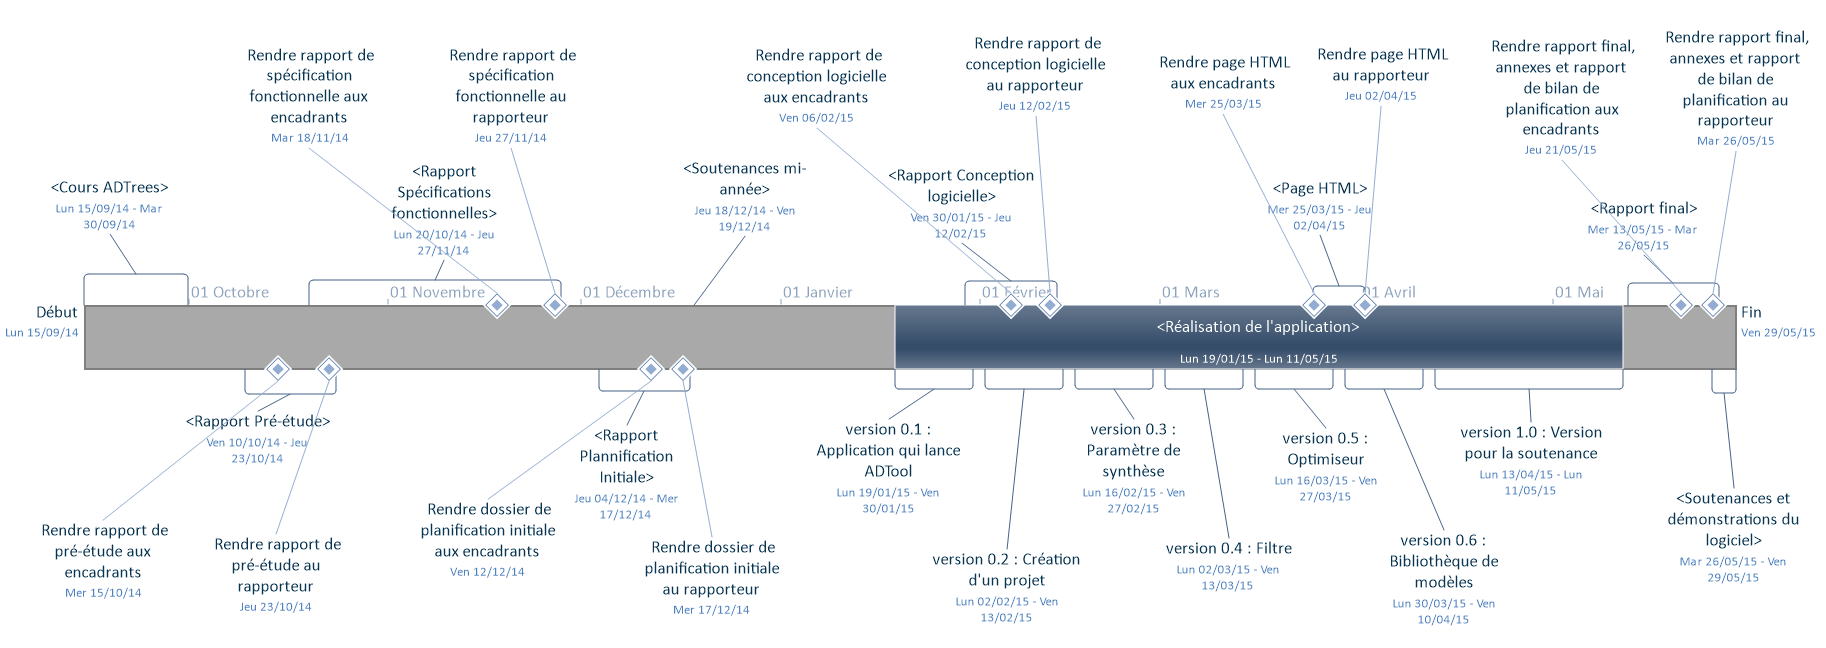
\includegraphics[height=0.60\textwidth]{figure/planification.png}
				\caption{Planification modélisée sous MS Project.}
				\label{fig:planif}
			\end{figure}
		\end{landscape}

	\subsection{Répartition des tâches}
		Au second semestre, seuls resteront Pierre-Marie {\sc Airiau}, Valentin {\sc Esmieu} et Maud {\sc Leray} à travailler sur ce projet, étant donné que le reste du groupe part étudier à l'étranger. Par conséquent, nous comptons séparer le travail ainsi :
		\begin{itemize} 
			\item l'un d'entre nous développera les fonctionnalités d'analyse de \glasir{} à proprement parler ;
			\item le deuxième se tournera plutôt vers l'intégration d'ADTool dans \glasir{} ;
			\item le troisième apportera les modifications à ADTool.
		\end{itemize} 
		Valentin suivant le deuxième semestre de la troisième année à partir de mi-janvier, cette répartition sera problablement affectée par les dates d'examens qui ne concordent pas entre la troisième et quatrième année. % faut il le dire ? 

